%!TEX root=main.tex
\subsection{Data Augmentation}
\label{sec:data_augment}

In this group of experiments, we study the effects of two specific data augmentation methods: \textit{GaussianBlur} and \textit{ColorJitter}. 

\begin{figure}[htp]
	\label{fig:data_augment_final}
	\begin{tabular}{cc}
		\subfloat[With Data Augmentation]{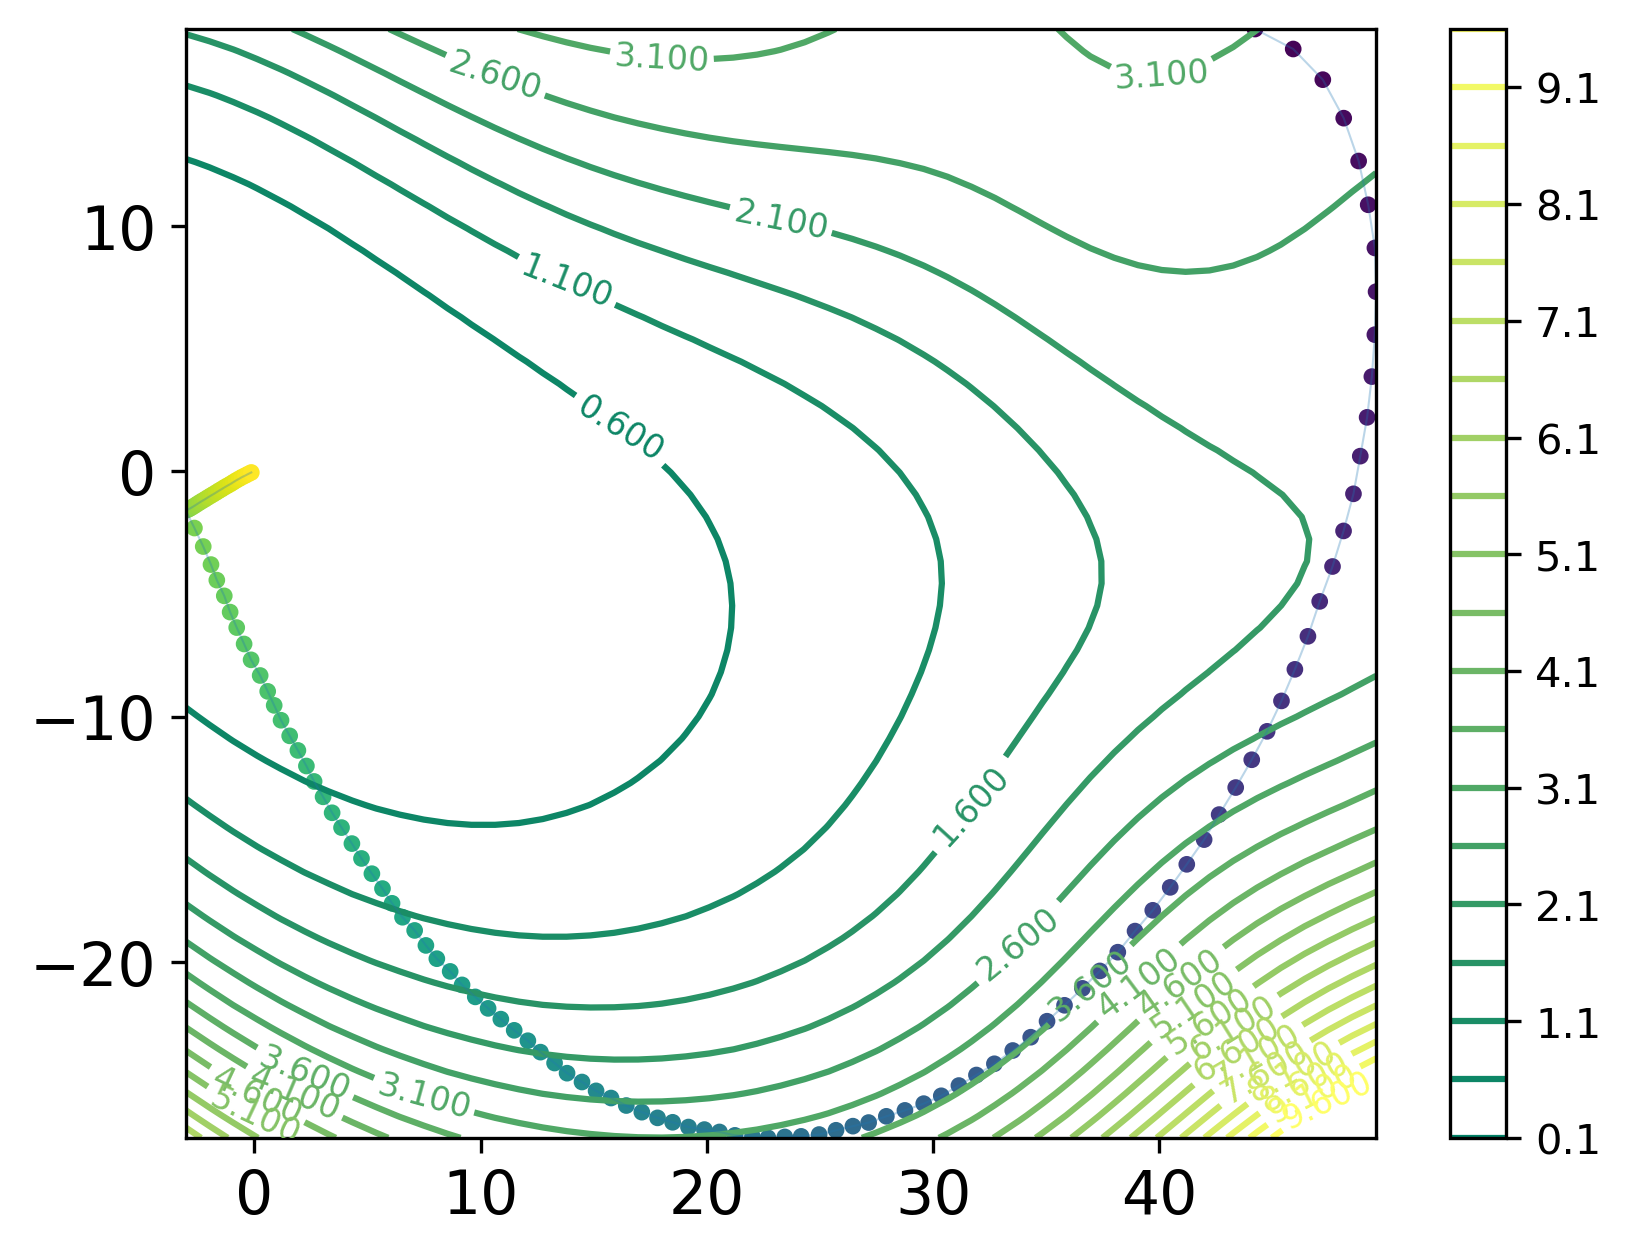
\includegraphics[width =  0.45\linewidth]{results/data_augment/resnet20_with_final.png}} &
		\subfloat[Without Data Augmentation]{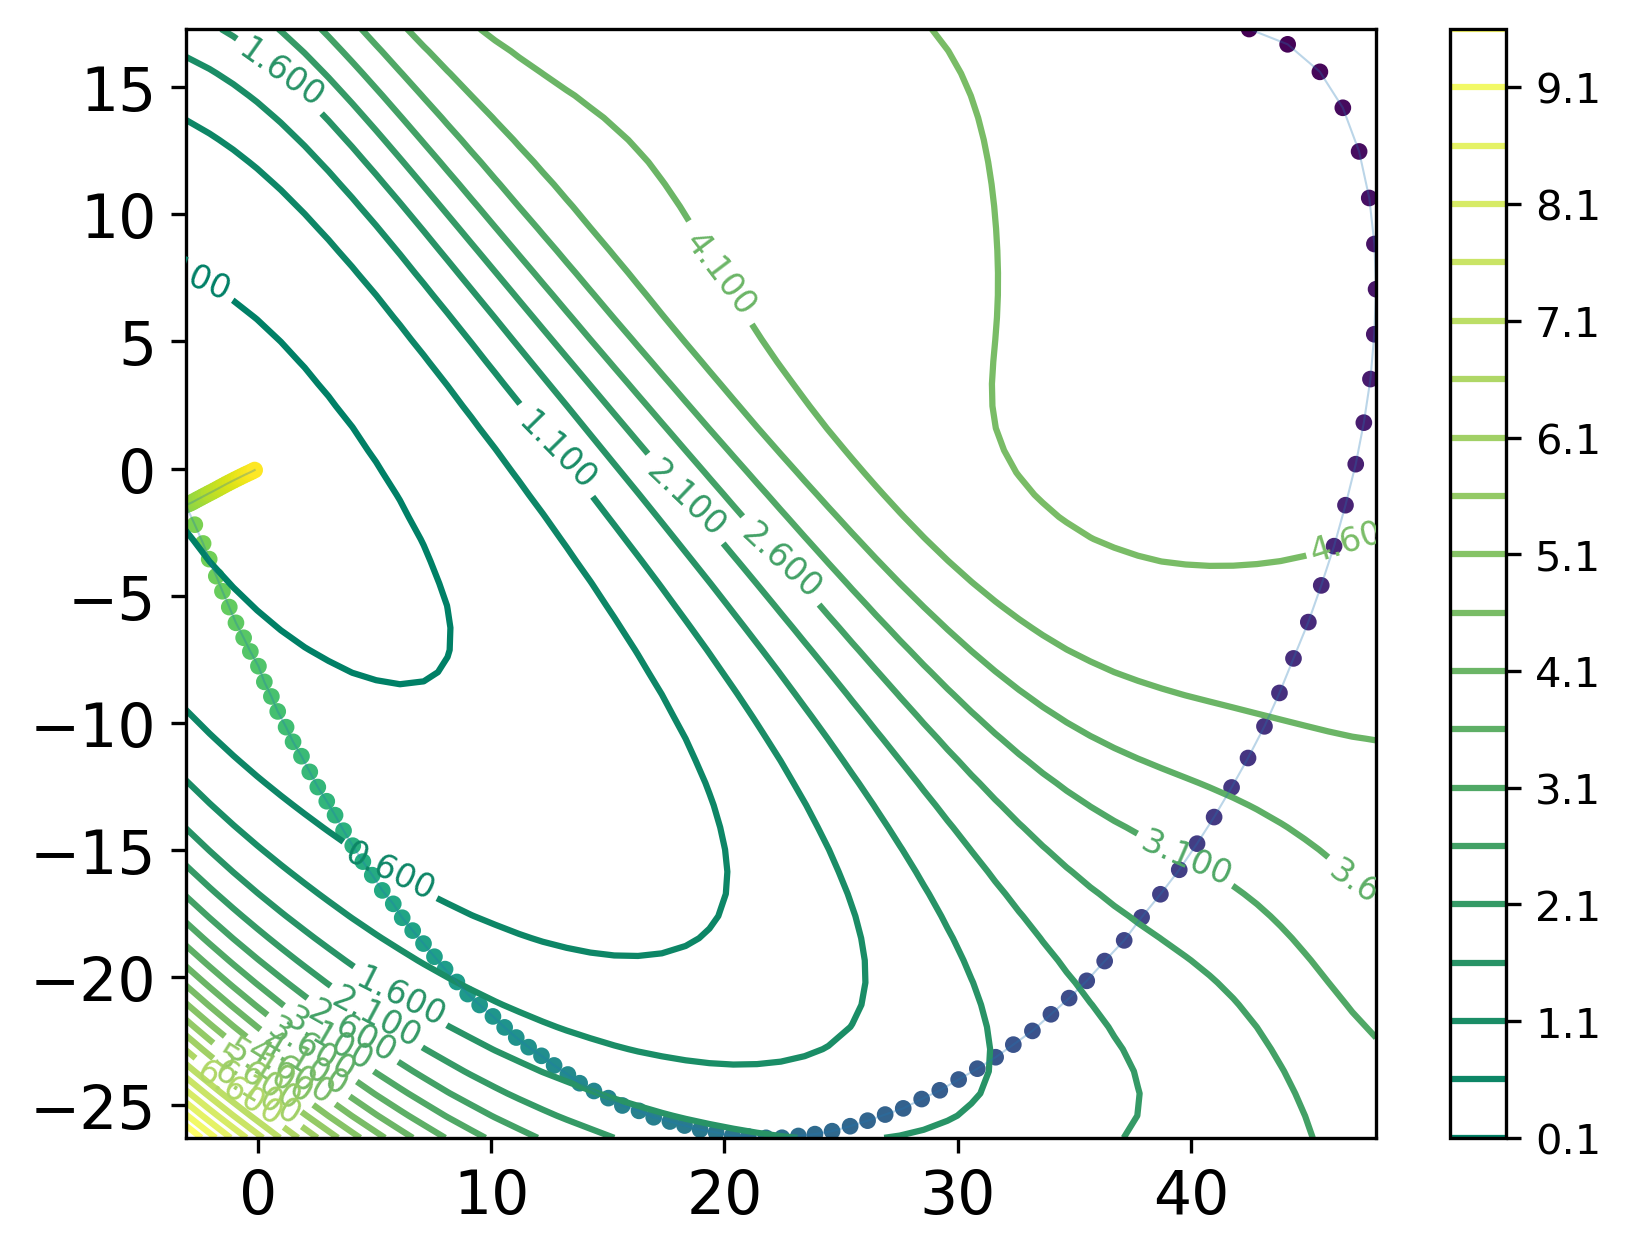
\includegraphics[width =  0.45\linewidth]{results/data_augment/resnet20_without_final.png}} 
	\end{tabular}
	\caption{Loss landscape with/without Data Augmentation (Trained)}
\end{figure}

Surprisingly, the extra data augmentation greatly improves the smoothness of the loss surface. 
